\subsection{Microsoft Academic Graph} \label{subject_indexing_mag}

The \acrfull{mag} is a knowledge base whose aim is to semantically relate scientific publications to one another \cite{shen2018web}. Its nodes can be of one of six types: publication, author, institution, journal, conference and concept. Having a high-quality concept model is detrimental and has been the main focus of Microsoft Research. The research group has developed throughout the past five years a concept hierarchy model which is used to semantically categorize scientific publications. Their pipeline comprises three steps. First, concepts are discovered; these concepts are then assigned to documents when semantically appropriate; finally, the relationships between the documents are used to build a concept hierarchy. We will now look at each of these steps more in detail.

\begin{table}
\begin{center}
    \begin{tabular}{| p{1.6cm} | p{2.9cm} | p{2.7cm} | p{2.3cm} |} 
    \hline
     & \thead{Concept \\ discovery} & \thead{Concept \\ tagging} & \thead{Hierarchy \\ building} \\ [0.5ex] 
    \hline\hline
    \thead{Problem} & \makecell{knowledge base \\ type prediction} & \makecell{multi-label text \\ classification} & \makecell{topic hierarchy \\ construction} \\ 
    \hline
    \thead{Solution} & \makecell{graph link analysis \\ on Wikipedia} & \makecell{word embeddings \\ + \\ graph structure} & \makecell{extended \\ subsumption} \\
    \hline
    \thead{Test \\ accuracy} & \makecell{94.75 \%} & \makecell{81.20 \%} & \makecell{78.00 \%} \\
    \hline
    \end{tabular}
    \caption{Summary of each phase of the \acrshort{mag} development.}
    \label{tab:mag}
\end{center}
\end{table}

Before introducing each of these steps, we explain the word embedding model they use, called skip-gram \cite{mikolov2013distributed}, which is the key component of their procedure. The word embeddings are trained by comparing them with the embeddings of the word that surround it in the text. Thus, embeddings are trained locally, focusing on the context of each word, rather than globally, where statistics and other metrics that consider the data as a whole are introduced.

After outlining \acrshort{mag}'s three steps, we introduce the two ways in which its data can be accessed. The \acrfull{makg} \cite{faerber2019microsoft} offers the data in RDF files, which are suitable for analysis tasks and efficient exploration. The second option is an expressive \acrshort{api}, provided by OpenAlex, which offers granular access to the documents and subjects. It also includes all the subject assignments, whereas the \acrshort{makg} only assigns fields. Therefore, we will use OpenAlex in this thesis.

\subsubsection{Skip-gram} \label{mag_skipgram}

The key component of Microsoft's approach is Skip-gram \cite{mikolov2013distributed}, a model for representing words as vectors, called embeddings. The embeddings are improved by training the model. The model receives the center word, and it should predict the context words. How many context words the model should be able to predict depends on the window size. We have implemented skip-gram in PyTorch\footnote{\url{https://github.com/carlosfranzreb/skipgram}}. Details about the training procedure and examples of embeddings can be found in section \ref{implementation_skipgram}.

Skip-gram arises as a counterpart to the \acrfull{cbow} model. This model is trained by giving it the words surrounding a certain word as input, called context words. It then has to predict the center word, i.e. the word that is surrounded by the context words in the data. Skip-gram was an improvement in both training time and semantic quality of the representation, according to the experiments of the authors \cite{mikolov2013efficient}.

The initial model was improved by adding two features. The first is subsampling of frequent words. The representation of words that appear often doesn't change much after a while, as the model has already tuned them. On the other hand, words that seldom appear on the data need more iterations for their representations to achieve a comparable accuracy. Therefore, frequent words are subsampled according to the formula below, which aggressively discards words whose frequency exceeds the threshold $t$. This increases accuracy, as the model doesn't overfit frequent words.

$$ Discard(word) = 1 - \sqrt{\frac{t}{freq(word)}} $$

The second improvement to the model was the introduction of negative sampling. It alleviates the computational cost of the problem, which, without negative sampling, requires computing the softmax of all data points. With negative sampling, we only consider $k$ words other than the input words, called negative samples. We assume that their vector representations should be considerably different from the representation of our input word. Thus, the model should output zero when fed the input word and one of the negative samples.
\subsubsection{Concept discovery} \label{mag_concept_discovery}

Given the vast amount of publications that appear every year (a number that doubles every dozen years \cite{dong2017century}), manually curating concepts is not a possibility anymore. A large amount of concepts is needed to properly characterize every document. Temporal dynamics (i.e. how research focus shifts over time) should also be monitored. This requires regular updates of the concept model, which again hinders the manual approach to solving the task.

Microsoft Research has adopted a hybrid approach for discovering concepts. They have manually defined the first two levels of the concept model (i.e. the two broadest levels) as well as 2000 other high-quality concepts, and solved the \textit{knowledge base type prediction} problem to assist them in discovering more specific concepts from the Wikipedia knowledge base. Their approach iterates between \textit{graph link analysis} for discovering potential concepts and \textit{entity type based filtering and enrichment}, which selects the most appropriate concepts out of the candidates retrieved in the previous step. The iteration is executed a few times, without any particular stopping criterion.

Graph link analysis explores concept candidates by assuming that the nearest neighbors of a concept are also concepts. Similarity between Wikipedia entities is defined based on the amount of hyperlinks to other entities that they share \cite{witten2008effective}. In the second step of the loop, the candidate concepts are filtered based on their type. Entities that belong to types which are irrelevant for the concept model, such as \textit{person}, are removed. Then, all other Wikipedia entities of the remaining types are added to the list of candidates. Which types are valid is determined using an undisclosed knowledge base.
\subsubsection{Concept tagging} \label{mag_concept_tagging}

Tagging concepts to publications is performed by solving a multi-label classification problem. Heuristics are applied to reduce the number of candidate pairs between concepts and publications, as evaluating every possible pair is unfeasible. All concepts of the first two levels as well as the concepts present in the publication's \acrfull{ert} are included in the classification task. The \acrshort{ert} is an extension of the text that describes an entity, termed \acrfull{srt}, to include textual information from its neighboring nodes in the \acrshort{mag}. Four representations of each \acrshort{ert} are concatenated and used as its vector representation: bag-of-words, bag-of-entities, embedding-of-words and embedding-of-entities. Words are also embedded as vectors using a skip-gram model \cite{mikolov2013distributed} that was pre-trained on an academic corpus.

To assign an \acrshort{ert} to each concept, the authors first manually assigned venues to concepts. The \acrshort{ert} of each concept is then the aggregation of the \acrshort{ert}s of the venues it was assigned. The mapping of venues to concepts is not available online. Once all publications and concepts are embedded (both as \acrshort{ert}s), a confidence score for each pair of concept and \acrshort{ert} is computed as the cosine similarity between their vector representations. The authors computed confidence scores for 50 billion pairs and kept one billion of them.
\subsubsection{Hierarchy building} \label{mag_hierarchy_building}

Once the publications have been tagged with the concepts, they can be used to extract a hierarchy for the concepts. The authors use \textit{subsumption} for this purpose, which assumes that concept $x$ subsumes concept $y$ if $y$ only occurs in a subset of the publications where $x$ occurs \cite{sanderson1999deriving}. The condition can be relaxed; $y$ is considered a child of $x$ in the hierarchy if both terms co-occur in a certain proportion of publications, i.e. 75 \%. The authors extend this method by including the confidence scores for the pairs of concepts and publications computed in the previous phase.

The resulting subsumption model was used to construct a six-level hierarchy of concepts. The relationships between the concepts of the first two levels were adjusted manually. All other relationships were left as they were output by the model. A limitation of this model, which translates to a worse accuracy (see table \ref{tab:mag}), is that relationships are not always transitive. For example, Fernando Alonso is a Formula 1 driver, which is a profession, but the relationship between ``Fernando Alonso'' and ``profession'' is unclear. The authors stated that they plan on addressing this issue by including information about the types of the entities.
\subsubsection{Updates since the paper's publication} \label{mag_updates}

Last year, the research group posted a blog post\footnote{\url{https://www.microsoft.com/en-us/research/project/academic/articles/expanding-concept-understanding-in-microsoft-academic-graph/}} highlighting some changes to the methods described above. There were two major updates to the phase of discovering concepts, which we discuss in this section. These two updates increased the number of concepts from 227 thousand to over 700 thousand. The second update is also performed regularly to discover new topics.

The first update consisted of adding concepts from the biomedical domain using the  Unified Medical Language System (UMLS) vocabulary. Biomedical concepts from the (UMLS) that were relevant to the corpus (regarding term frequency) were added to the concept model. This procedure was performed only once. The second update is the paradigm shift for topic discovery. Instead of retrieving concepts from Wikipedia, the new approach directly extracts concepts from the academic literature. It consists of two steps.

\begin{enumerate}
    \item Identify words or phrases in the text of the publications that are concepts (without stating which specifically). This problem is called \textit{sequence labeling}. The authors' approach consists of doing lexical matching on a sample of \acrshort{mag} publications using the synonyms of existing concepts to generate a training set. This set is then fed to a transformer as a context encoder and a conditional random field as a tag decoder to train a binary classifier on each word.
    \item Differentiate between existing, new and low-quality concepts by evaluating the relevance of the URLs returned by the Bing Web Search \acrshort{api} when looking for the concept. Equivalent concepts are grouped together.
\end{enumerate}

\subsubsection{Accessing the data} \label{mag_access_data}

Microsoft provides \acrshort{api} access\footnote{\url{https://docs.microsoft.com/en-us/academic-services/project-academic-knowledge/reference-evaluate-method}} to their corpus, including already tokenized abstracts and the subjects of each document. A subscription is required to access the \acrshort{api} endpoint and the rate limit is set to 10,000 transactions per month and 1 per second. Unfortunately, the \acrshort{mag} service was shut down at the end of 2021. We therefore discuss two other options, that also offer \acrshort{mag} data, in the following sections. We then close this chapter by arguing our choice between them.

\paragraph{MAKG} \mbox{}

Michael Färber has processed the data from the papers and offers dump files in \acrfull{rdf} format \cite{faerber2019microsoft} and also provides an SPARQL endpoint\footnote{\url{https://makg.org/sparql}}. Each file includes different information, such as metadata about the subjects, the authors or the papers. The abstracts have also been reconstructed into free text, as Microsoft only provides them as lists of tokens.

Färber's dumps comprise over 238 million publications and 740,460 subjects\footnote{These numbers refer to the dump of 29.05.2020}. How the subjects are distributed among the fields (i.e. the subjects of the first level) is displayed in figure \ref{fig:subjects_per_field_per_level}. This plot only considers the subjects that are part of the hierarchy. There are 196,631 subjects (27 \%) that do not belong to any of the fields.

341,959 subjects of the hierarchy (46 \%) belong to the fields of biology and medicine. Environmental science is the least represented field, with only 126 subjects, followed by history, which comprises 1,510 subjects. Regarding the levels, there are 19 subjects in the first level (called fields from now on) and 292 in the second. The latter ones include over 100,000 subjects per level, incrementally increasing and peaking at 165,321 subjects in the sixth level.

\begin{figure}
    \centering
    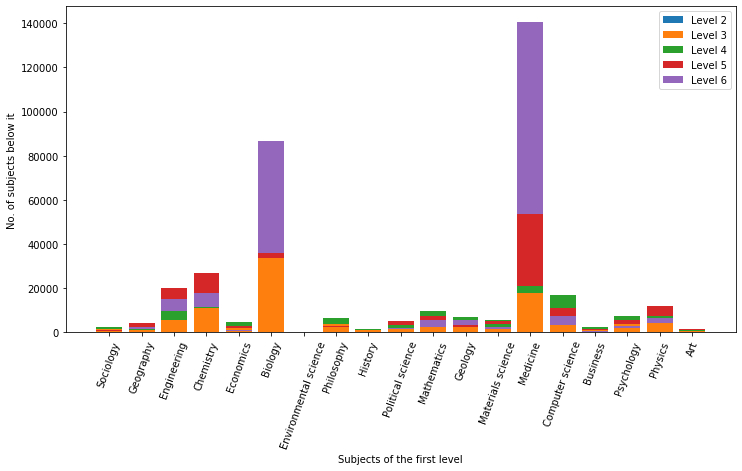
\includegraphics[width=\textwidth]{figures/related_work/makg/subjects_per_field_per_level.png}
    \caption{Subjects present in the MAKG.}
    \label{fig:subjects_per_field_per_level}
\end{figure}

\begin{figure}
    \centering
    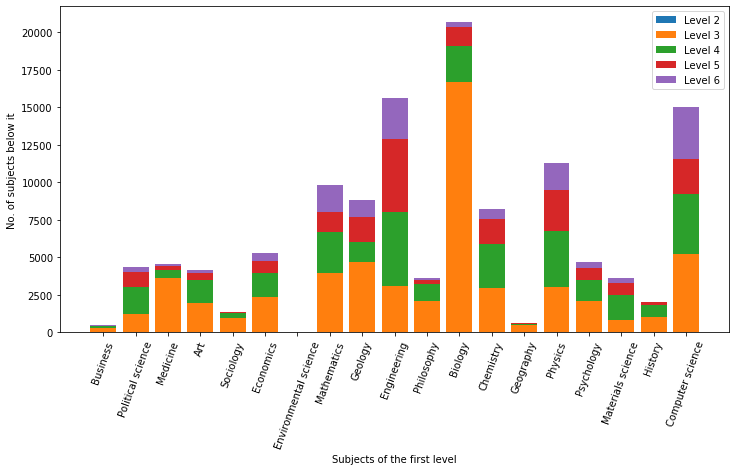
\includegraphics[width=\textwidth]{figures/related_work/makg/subjects_w_article.png}
    \caption{Subjects of the MAKG that have a Wikipedia link.}
    \label{fig:subjects_w_article}
\end{figure}

\begin{figure}
    \centering
    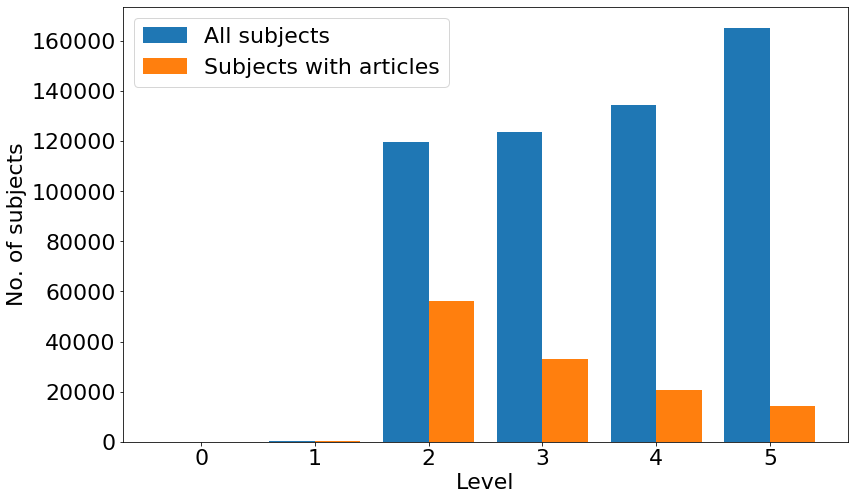
\includegraphics[width=.75\textwidth]{figures/related_work/makg/subject_distribution_comparison.png}
    \caption{Comparison of all subjects with the subset that have a Wikipedia link.}
    \label{fig:subject_distribution_comparison}
\end{figure}

124,385 subjects (17 \% of all subjects) have a Wikipedia link. These are shown in figure \ref{fig:subjects_w_article}. They are relevant for computing the vector representations of the subjects. If they are not present, we cannot do so, as we don't have a text associated to the subject we can use for the vectorization procedure. Biology is the field with the most links, followed by Computer Science and Engineering. Only 4,574 subjects of the 179,741 in the field of Medicine (2.5 \%) have a link, which is why this field is no longer the most populated field when considering Wikipedia links. The difference among all subjects and those with links is shown in figure \ref{fig:subject_distribution_comparison} on a per-level basis. When looking at all subjects, the number increases with the level. When looking at the subjects with links, the opposite occurs: the number of subject decreases with the level.

Regarding the subject assignments of the documents, Färbers files don't include all the subjects assigned to each document. When querying the SPARQL endpoint for all subjects that have been assigned to at least one paper, only 19 subjects are returned. They are very broad subjects, such as \textit{Geology} or \textit{Computer Science}. The assigned subjects in Färbers \acrshort{rdf} files also don't always coincide with the ones assigned by Microsoft. For example, in the \acrshort{rdf} files the paper \textit{Determination of vitamin D3 and 25-hydroxyvitamin D3 in foodstuffs by HPLC UV-DAD and LC–MS/MS} has the subject \textit{Environmental Science}, whereas in Microsoft Academic the topics assigned to the publication include \textit{Vitamin}, \textit{High-performance liquid chromatography} and eight others. These subjects can be retrieved through the \acrshort{api}.
\paragraph{OpenAlex} \mbox{}

OpenAlex\footnote{\url{https://openalex.org/about}} is the successor of the \acrshort{mag}. It offers the whole \acrshort{mag}, combined with several other sources, through a RESTful \acrshort{api}. It arose because the \acrshort{mag} was shut down by Microsoft at the end of 2021, which opened the door for other companies to fill the gap. OpenAlex is still on beta release, which they plan to emerge from in the upcoming months. However, it currently has all the data that \acrshort{mag} had, and more. It also imports data from sources like Crossref\footnote{\url{https://www.crossref.org/}}, ORCID\footnote{https://orcid.org/} and PubMed\footnote{https://pubmed.ncbi.nlm.nih.gov/}.

Among numerous interesting features, it allows searching for publications that are assigned a certain subject. When retrieved from the API, subjects includes the \acrshort{api} request to retrieve its corresponding publications, as well as the number of publications it is assigned to. We can use this number to assess the relevance of a subject. Subjects also include a list with all its ancestors, which we can use to navigate the hierarchy. The \acrshort{api} offers several filters when querying subjects, such as hierarchy level and ancestors.
\paragraph{Choice of data source} \mbox{}

The two options, \acrshort{makg} and OpenAlex, offer different services. \acrshort{makg} stores the \acrshort{mag} data as \acrshort{rdf} triples, which are suited for exploring the knowledge graph through its entities, integrating the \acrshort{mag} data with other sources and performing large scale data analysis \cite{faerber2019microsoft}. OpenAlex, on the other hand, offers a variety of filters to construct granular \acrshort{api} requests, which makes the data very accessible. However, it is not as scalable as the \acrshort{makg}, which can be navigated efficiently with SPARQL.

The main drawback of \acrshort{makg}, which renders it useless for our use case, is that it does not include the assignments of subjects to documents. It only includes the assignment of publications. We require these assignments to build a dataset of documents and their assigned subjects, which we then use to train a supervised classifier. OpenAlex does offer all the assignments that are present in \acrshort{mag}, and therefore is our choice as the data source for subjects and training data. Given that we only require basic filtering and don't want to perform any large scale analysis, we do not require the scalability that \acrshort{rdf} triples offer. The \acrshort{api} objects that OpenAlex outputs fulfill all our requirements.

